\documentclass{beamer}
\usepackage{amsmath,amsfonts}	% use math symbols
\usepackage{graphicx} % insert images
\usepackage{url} % insert urls
\usepackage{textpos} % package for the positioning
\usetheme{Ilmenau} % change theme


\begin{document}

%% MAKE TITLE
\title{Learning from Causation}
\subtitle{Fundamental of Casual Inference and its Applications}
\author{Huang Xiao} %\\ \small{xiaohu@in.tum.de} }%\thanks{Funded by ARAMiS project}}
%\and Author2 \inst{1} }
%\and Author3 \inst{2}}
\institute[Technische Universit\"at M\"unchen]
{ 
	%\inst{1} 
	Chair of IT Security (I20) \\Department of Informatics \\Technische Universit\"at M\"unchen 
	%\and
	%\inst{2} Cloud Service Lab\\Fraunhofer AISEC
}

\date{\today}
\maketitle

%% CHANGE THE DEFAULT TEMPLATE
% position the logo
\addtobeamertemplate{frametitle}{}{%
\begin{textblock*}{100mm}(0.98\textwidth,-0.7cm)

\includegraphics[height=0.53cm,width=0.9cm,keepaspectratio]{imgs/TUM}
\end{textblock*}}

\AtBeginSection[] {
	\frame<beamer>{ 
		\frametitle{Overview}   
		\tableofcontents[currentsection] 
 	}
 }
 % add frame number
%\setbeamertemplate{footline}{%
  %\raisebox{5pt}{\makebox[\paperwidth]{\hfill\makebox[10pt]{\scriptsize\insertframenumber}}}}

%% START PRESENTATION
\section{Fundamental of Causal Inference}
\subsection{Motivation}
\begin{frame}{What is Causality?}
\begin{block}{A definition from Wikipedia}
\textbf{Causality} (also referred to as causation) is the relationship
between an event (\textit{the cause}) and a second event (\textit{the effect}),
where the second event is understood as a consequence of the
first.
\end{block}\pause
\textbf{An example in real life} : Does smoking cause lung cancer?\\
\pause	
\begin{center}
\alert{Yes, it might be!}
\end{center}
\end{frame}
\begin{frame}{From Probabilistic View }
\textbf{Problem:} Does smoking cause lung cancer?\pause
\begin{center}
\begin{itemize}
\item Smoking does \alert{increase the probability} of getting lung cancer.
\end{itemize}
\end{center}
\end{frame}
\begin{frame}{Statistical Inference Overview}
\begin{figure}
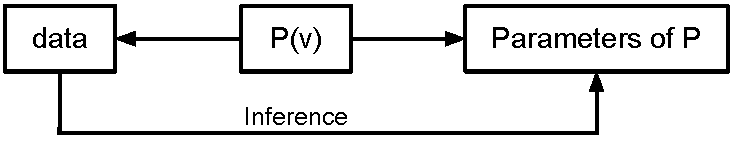
\includegraphics[scale=0.7]{imgs/statInf}
\end{figure}
\begin{itemize}
\item Approximate an estimate of $X$ given evidence $e$, namely, $Pr(X\,|\,e)$. E.g., Regression or Classification problems.
\item Rejection of hypothesis, i.e., assert wether samples are from a certain distribution.  
\item Confidence interval, i.e., construct an interval based on dataset 
\end{itemize}
\end{frame}
\begin{frame}{Causal Inference Overview}
\begin{figure}
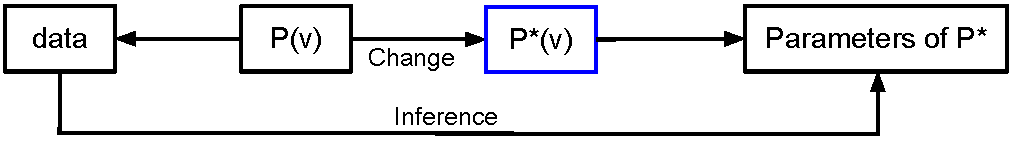
\includegraphics[scale=0.6]{imgs/causalInf}
\end{figure}
\begin{itemize}
\item What if $P$ has shifted itself to $P^*$?
\item<2-> \textbf{Key factors:} Causes, Changes, and Invariants . 
\item<2-> Inference of $P^*$ and reasoning of changes. 
\end{itemize}
\end{frame}
\begin{frame}{What makes Causal Inference interesting?}
\begin{itemize}
\item Human understands the world in terms of causes and effects.
\item Empirical science is about establishing causes.
\item Causal inference gives a mathematical language for causal
statements, and tools to solve causal problems formally.
\item Alternative exercising to decision making, reasoning, etc.
\end{itemize}
%\begin{alertblock}{Note}
%Causal Inference has fundamental difference with machine learning
%\end{alertblock}
\end{frame}
\subsection{Causal Graphical Model}
\begin{frame}{Association}
\begin{itemize}
\item Now we want to find out what \alert{causes} lung cancer
\end{itemize} \pause
\begin{columns}
\begin{column}{0.5\textwidth}
\begin{table}
\centering
\begin{tabular}{|c|c|c|c|}
\hline
& & \multicolumn{2}{|c|}{Lung cancer}\\\hline
smoking & yellow teeth & yes & no\\\hline
yes & yes & 100 & 400\\\hline
yes & no & 100 & 400\\\hline
no & yes & 1 & 450\\\hline
no & no & 9 & 8540\\\hline
\end{tabular}
\caption{Data observations from 10000 people}
\end{table}
\end{column}\hfill
\begin{column}{0.5\textwidth}
\vspace*{-0.5in}
\begin{figure}
\centering
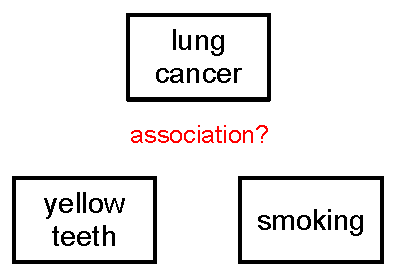
\includegraphics[scale=0.6]{imgs/smokepl}
\end{figure}
\end{column}
\end{columns}
\end{frame}
\begin{frame}{Measurements of Association}
\textbf{To find out associations among variables}
\begin{itemize}
\item Mutual information (Information theory)
\item Pearson (linear) correlation
\item Spearman's rho (rank correlation)
\item Effect size between two variables
\item Many others
\end{itemize}
\end{frame}
\begin{frame}{Observations from Data}
\textbf{Obviously}
\begin{itemize}
\item \textit{yellow teeth} and \textit{lung cancer} are associated.
\end{itemize}\pause
\alert{\textbf{But...}}
\begin{itemize}
\item Bleaching the teeth does not help reduce the probability
of getting lung cancer.
\end{itemize}\pause
\begin{alertblock}{Caution!}
Correlation does not imply Causation
\end{alertblock}
\end{frame}
%% START NEW SECTION
\section{History}

\begin{frame}{History}

\begin{itemize}
\item Discuss the history of the problem.
\item Describe context for the problem.
\item Outline prior work on the problem.
\end{itemize}

\end{frame}



\section{Representation}

\begin{frame}{Representation}

Represent the problem in symbolic, graphic, or numeric format.

\bigskip

Mathematical formulas may be typeset:
\[ \int_0^\frac{\pi}{2}\frac{1+\cos 2x}{2} \: dx \]

\end{frame}



\section{Methods}

\begin{frame}{Methods and Tools}

Discuss technical methods or tools required to formulate and solve the problem mathematically.

\bigskip

\begin{theorem}
If $f$ is continuous on $[a,b],$ then
$$\int_{a}^{b} f(x) \: dx = F(b) - F(a)$$
where $F$ is any antiderivative of $f,$ that is, a function such that $F' = f.$
\end{theorem}

\end{frame}



\section{Solution}

\begin{frame}{Solution of the Problem}

Present a solution of the problem, perhaps for a simple case, and indicate how the solution may be achieved in other cases.

\bigskip

\begin{example}
\[ \int_0^\frac{\pi}{2}\frac{1+\cos 2x}{2} \: dx=\frac{\pi}{4}  \]
\end{example}

\end{frame}



\section{Conclusion}

\begin{frame}{Conclusion}

Summarize the information presented in the talk.

\bigskip

\begin{itemize}
\item Problem statement
\item Relevance
\item Mathematical tools
\item Solution
\end{itemize}

\end{frame}




\section{References}

\begin{frame}{References}

\begin{thebibliography}{99}
\bibitem{Boas} R. P. Boas,  Can we make mathematics intelligible?  \textit{Amer. Math. Monthly}, \textbf{88} (1981), 727--731.

\bibitem{Page} M. E. Page,  A Brief Citation Guide for Internet Sources in History and the Humanities (Version 2.1),
\begin{url}http://h-net.msu.edu/$\sim$africa/citation.html\end{url}.

\end{thebibliography}

\end{frame}





\end{document}